\chapter{Evaluation}\label{chapter:evaluation}

After illustrating the system designed and developed, this chapter evaluates this system in real user study and shows and discusses the the results.

\section{Motivation and Goals} \label{sec:mg}

Initially, recommender systems are usually evaluated based on their prediction accuracy - how accurately they can predict the items that the users are most interested in. However, it is now widely agreed that accuracy is an important but not unique measurement for the quality of recommender systems, because the user is not always looking for the best predictions of their tastes. Especially in cases where the user does not have specific preferences in mind and is still in the exploration stage, users may value more the diversity and novelty of the recommendation. Moreover, if the recommender system is built on a mobile system, the user is usually less patient when using the system. Decision effort that is needed in finishing a task is also an influential factor for the quality of the recommender system. Thus, besides the evaluation of prediction accuracy, user's decision effort and user's general satisfaction of the system should also be measured. Especially concerning the context-aware feature,  whether the user is well aware of the benefits of context and the corresponding context-aware explanations should also be measured.

There are three different types of evaluation experiments: offline, user studies and online experiments \cite{ref:35}. Usually performing offline experiments is the easiest way because no user is involved. Through using existing data sets and a protocol that models user behavior, recommender system performances such as prediction accuracy can be easily measured at low cost. However, because the narrow set of properties it can measure, and the fact that it is difficult to create a reliable simulation of user interactions with the system \cite{ref:35}, this approach is not appropriate for the system in this thesis. A more expensive option is the user study, where a small number of users are asked to perform a set of tasks using the system. A set of raw metrics are measured during the task for future statistical analysis and users usually need to answer a set of questions about their feelings of the system. This type of experiment provides a controllable experiment environment so that it can be adapted and used to measure different properties. It is suitable for recommendation approaches that rely on the interaction of users with the system. Finally, for realistic recommender systems, online evaluation can be used where the performances of real users are evaluated when they are using the system and are not aware of the ongoing experiment. However this approach can not be adapted easily to specific evaluation requirements. Based on all the discussions above, the user study experiment was adopted for the evaluation of the system in this thesis.

Two variants of the system were tested. The baseline system is presented in Section \ref{sec:rs_bs}. To test all candidates within subjects method was used, where each subject tests a set of candidates on different tasks \cite{ref:36} so that the two system variants can be more reasonably compared to each other. However, the same people testing both variants can introduce biases due to for example learning effect (e.g., the user may spend less time on the second tested variant because she/he become more familiar with the interface after using the first variant.). To avoid such bias, the order of variants to be tested by the user should be randomized and enough time should be left to let the user get familiar with the system before the task. Moreover, the case base (knowledge base) is kept fixed in the evaluation so that the recommendations are all based on the same foundation.

When drawing conclusions from the experiments, it was hoped that the conclusions can be applied to general cases rather only to the context of the experiments. To increase the probability of generalization of the results, firstly, the experiment participants should represent as closely as possible the true population of users of the real system. In this evaluation, people of various ages (from 21 to 56) and occupations (e.g., freelance, student, teacher and software engineer) are invited to participate in the user study so that the test results can be as much generalized as possible. It was aimed to look for around 30 participants so that the number of sample data can be big enough to be evaluated using a paired t-test. To not overwhelm and exhaust the candidates, the experiment will be controlled in 10 to 15 minutes.

\section{Data Set} \label{sec:ds}

\subsection{Data Set for Clothes Items} \label{sec:ds_ci}

In this evaluation, data set retrieved in section \ref{sec:acr} will be used as the sample data. The extracted data is from online store Zalando as was introduced before. Those clothes items may not be actually available offline here in Germany. However for the evaluation purpose, they will be randomly assigned to a list of offline stores available in Germany. 

After the raw data was retrieved, it was preprocessed to get rid of irrelevant categories such as "Home" and "Child". The depth of the initial category tree was five and in this thesis only the category information up to depth two was kept and some of the categories that are similar to each other but have different names were merged to avoid sparsity problem. For example, "Lingeire \& Nightwear" in women's clothes category was merged with "Underwear" in men's category. So finally, 14 categories were defined: tops, dresses, underwear, cardigans, trousers, coats, blouses, jackets, skirts, jeans, socks, swimwear, suits and shirts. Then for each clothing item, irrelevant information was removed and the following information was kept:
\begin{itemize}
	\item{a numeric identifier (id),}
	\item{the clothes name,}
	\item{the price (in Euro, stored unit-less),}
	\item{one of 34 colors,}
	\item{one of 12 brands (including the sub brands such as "QS by s.Oliver"),}
	\item{the sex,}
	\item{one of 14 types of clothes,}
	\item{the link to an image of the item}
\end{itemize}

The result set contains 3920 items in total with 2238 clothes items for female sex and 1682 clothes items for male sex. For each clothing type there are between  ???

\subsection{Data Set for Context Case Base} \label{sec:ds_ccb}

As was mentioned in previous section, the case-based context-aware recommender system developed in this thesis recommends based on a case base which can be built up through collaborative as well as expert-driven approach. For the evaluation in this thesis, expert-driven approach was used to first set up a starting case base. Since the users were asked to make purchasing decisions while imagining themselves being in a certain context scenario, the starting case base should be as various as possible for the corresponding scenarios. Take buying clothes for sports purpose for example, user's potential choice may vary from sports trousers, sports shirts to swimming suits and yoga pants. Apparently, it can be difficult to find enough people with choices vary enough for the case base in a short period of time, it was believed to be easier and more efficient to use expert-driven knowledge acquisition approach.

Clothes selection was done for each of the five predefined context scenarios that were used in the evaluation task, for which both common sense and the Zalando website were used as the main resources. For example, according to the common sense, thick clothes such as jacket, sweater, long trousers, coat will be selected for cold weather and clothes such as dresses will be selected for party purpose. On the other hand,  in the Find your style page\footnote{http://www.zalando.co.uk/styles/} in Zalando website, different styles such as going out, romantic, casual, business are defined and they were also used as references for the selection of clothes for the case base. In total, ten cases were added for each context scenario with five cases for men and five cases for women. 

\section{Test Setup} \label{sec:ts}

In the baseline system, the system recommends without initial preferences from the user. To optimize the initial recommendation quality,  a set of items are selected using a diversity-enhanced technique to ensure the coverage of the presented items. Compared to that, the system developed in this thesis tries to improve the the initial recommendation through integrating complex contextual information into the recommendation algorithm. So the baseline system is a simplified version of the developed variant. It does not consider contextual information during recommendation and does not contain the context setting UI in Figure \ref{fig:contextSettings1}. However for both systems, the user can critique on items features and iteratively update the recommendations according to their personal interests. 

The test hardware is a 3.7 inch 480 x 854 resolution Android smartphone (Motorola DEFY) running the Android operating system of version 2.3.7.

\subsection{Testing Framework} \label{sec:ts_tf}

In this evaluation, the testing framework follows the one presented in paper \cite{ref:5} and the recommendation quality was mainly qualitatively measured with a standard questionnaire. Quantitative information was also collected to better interpret the result \cite{ref:35, ref:46}. The measured data was divided into four areas: prediction accuracy, decision effort, explanation benefits and context benefits.

\subsubsection{Prediction Accuracy} \label{sec:ts_tf_pa}

Prediction accuracy is by far the most discussed and the most important property for recommender system evaluation. It is based on a basic assumption that a system that provides more accurate predictions will be preferred by the user \cite{ref:35}. It measures the ability a system can help users find the items they like. In this thesis, this property was measured qualitatively by asking the user which system suggests more appropriate clothes. The appropriateness here reflects the accuracy of the recommendations. 

\subsubsection{Decision Effort} \label{sec:ts_tf_de}

People usually want a recommender system with high prediction accuracy and low decision effort. However, strategies yielding more accurate choices are often more effortful, but simple strategies can lead to lower levels of accuracy \cite{ref:38}. Especially in mobile exploratory scenario, a recommender system that is accurate but takes longer time or a lot of cognitive effort to reach the goal is also not useful. Thus in this evaluation, the decision effort was measured using both qualitative and quantitative methods.

\textbf{Quantitative Measurements} The decision effort can be quantitatively measured by the task time and the interaction effort. Task time is the time a user needs to find and select an ideal item after she/he is presented with the initial recommendations. Interaction effort here can be represented by the number of critiquing cycles. One critiquing cycle is counted when the user issues a critique on the item features, triggering the selection of new recommendations.

\textbf{Qualitative Measurements} The decision effort is also measured quantitatively by asking the user to rate the easiness of finding the information she/he needs using the system and asking the user the effectiveness of the system in helping her/him to complete the scenario. The scenario here means giving a context scenario, finding an ideal item to buy.

\subsubsection{Context Benefits} \label{sec:ts_tf_cb}

In spite of the goal of improving the quality of the recommendation, the integration of contextual information into the system also provides a new way for the user to personalize their recommendations. To study whether or not the user is interfered by the extra step of context setting and whether or not the user is aware of the benefits of context-aware recommendation, the user was asked does she/he understand the benefits of using contextual conditions.

\subsubsection{Explanation Benefits} \label{sec:ts_tf_eb}

From the user's perspective, explanation is an important experience because it helps the user understand how the recommender system work. Explanation is supposed to have many benefits including improving the transparency of the system, increasing the trust of the user to the system, persuading the user to try or buy the recommended item, etc. So in this evaluation, users were also studied to see whether they were aware of the explanation benefits through asking them whether they think the contextual explanations are useful. The clearness of the contextual explanations was measured qualitatively by asking the user whether she/he is satisfied with the provided contextual explanations and whether the contextual explanations provided by the system are clear.

\subsection{Testing Procedure} \label{sec:ts_tp}

The actual testing procedure used in the evaluation was structured as follows:

\begin{enumerate}
\item{Introduce the application to the user.}

Because the users were of different knowledge backgrounds, not all of them were familiar with terms like "recommender system" or "context". Since most of them had online shopping experiences before, to let the user quickly learn the concept of recommender system and the core functions of this application, websites like Amazon were used as real life examples to help the user gain a quick feeling of what the application does.

After the user understood the basic idea of the application, she/he was explained how to use it. Nowadays, mobile applications usually show a quick graphic instruction to tell the user how to use the system when they are first launched. Here a manual instruction was given with the same purpose.

\item{The user was asked to play around with the application.}

Before starting the evaluation task, the user was asked to play around with both variants of the system and ask questions whenever they were confused. They were asked to finish a simple task (i.e., select an ideal item using the current system). Usually, more questions would come out when they were trying to finish this simple task. In this way, it could be made sure that during the formal study, the user could focus on the task itself but not figuring out how to use the system.

\item{Explain the task setting to the user.}

There were two variants of the system as was introduced before. When testing with both variants, the user was asked to select an item she/he was most satisfied with while imagining her/himself being in a context scenario that was randomly selected by the system from a set of five pre-created context scenarios. A typical context description could be:

\blockquote{Imagine that you want to buy clothes for daily wear, you are a budget buyer and the temperature is cold.You don't care the exact location of the clothes.}

For each context, usually four factors were included. To see the full list of those scenarios, please refer to Appendix \ref{appendix:cs}. The user was first explained to the concept of context and then shown to the descriptions of the context scenarios that would be randomly selected during the user study. In this way, the user could get a full view of the study, feel more in control of the study and feel more confident in her/his actions.

The amount of advantages or disadvantages of context-aware recommender system compared to non context-aware recommender system might vary among different pre-created context scenarios. To avoid this bias, for each user study, the two system variants were tested using the same randomly chosen context scenario so that they could be compared under the same controlled situation. 

One thing that needs to be pointed out is that because in the formal study, when users were using the context-aware variant developed in this thesis, they didn't need to configure the context settings by themselves and the system would be automatically configured to be in the chosen context scenario. Because for pre-defined context scenarios, the context conditions such as the weather or the temperature could be different from the current one, thus must be programmatically set and could not be automatically retrieved from third party services. In some cases, the user might forget the existence of the context setting step. To avoid this situation, users were especially asked to use the context setting function and see the reaction of the system (updating of the item list) according to the change of their context settings. With this extra step, it could be made sure that they understand how the context-aware system works. They were also explained carefully the reason why they didn't need to configure the context in real user studies.

\item{Conduct the task.}

Once the user understood the task mentioned above, a variant of the application was set up and handed back to the user. After the user selected one item, she/he was given to another variant and asked to do the task again. To reduce the effect of learning curve, the order of the first variants to give was randomly selected. The user was also encouraged to give oral feedbacks during the task. 

At first the testing procedure was designed to ask the user to test each variant of the system twice, each time with a different context scenario, so that the user could be aware of the different reactions of these two variants when context changed. However, considering that this procedure design was too time consuming, with the goal of not overwhelming the user, this design was given up and the current procedure design was adopted.

\item{Finish the survey.}

After the user tested on both variants, she/he was asked to fill out a survey. The survey was created online using google form so that the user could fill it out privately. In this way, the influence of the interviewer could be reduced the most. These questions were extracted and adapted to our evaluation from the IBM Computer System Usability Questionnaire [37] and included the following statements:

\begin{itemize}
\item{Q1: It was easy to find the information I needed. }
\item{Q2: The system is effective in helping me to complete the scenario. }
\item{Q3: I like using this system.}
\item{Q4: I understood the benefit of using the contextual conditions. }
\item{Q5: I am satisfied with the provided contextual explanations. }
\item{Q6: I believe that the contextual explanations are useful.}
\item{Q7: The contextual explanations provided by this system are clear. }
\item{Q8: Which system do you prefer?}
\item{Q9: Which system suggest more appropriate clothes?}
\end{itemize}

Statements 4-7 were provided only for the context-aware version. Statements 4-7 were asked for both variants. At the end of the survey, the user was asked which system she/he preferred (Q8) and which system suggested more appropriate points of interest (Q9).The user could express a level of agreement to the statement ranging from 1 (strongly disagree) to 5 (strongly agree). 

\end{enumerate}

\section{Results} \label{sec:results}

This section analyzes the data collected in the user study for each property measurement.

\subsection{Participants} \label{sec:results_p}

For the study, participants of various age, religion, nationality, knowledge background and current profession were looked for. Overall a number of 23 people participated the user study, among which 17 people were students as well as employees in academia in fields including Computer Science, Electronic Engineering, Finance, Economics, and other 6 people were employees and freelancers from outside of the university. The average age was 27, with a maximum of 56 and a minimum of 21.

\subsection{Overview} \label{sec:results_o}

The measurements for decision effort and system preference for both two systems (CW denoting the variant using context-aware recommendation, NCW the one recommending without contextual information) are shown in Table \ref{tab:overview}. Next to the mean is the standard deviation and the last column denoting the p-value of a one-tail paired t-test with 22 degrees of freedom (23 participants - 1).

In the following sections, a detailed discussion of the measurements of the four properties (prediction accuracy, decision effort, explanation benefits and context benefits), the general system preference as well as the informal feedback will be given.

\begin{table}[H]
	\centering
	\caption{Overview of the result.}
	\label{tab:overview}
	\small
	\begin{tabular}{p{0.6in}p{1.2in}p{0.5in}p{0.5in}p{0.5in}p{0.5in}p{0.5in}}
	           \hline
		 &  & CW &  & NCW \\ 
 		 &  & mean & stdev & mean & stdev & p value \\ \hline
		 Decision Effort & It was easy to find the information I needed. & 3.74 & 0.92 & 3.61 & 1.16 & 0.3 \\ 
		Decision Effort & The system is effective in helping me to complete the scenario. & 4.09 & 0.79 & 3.74 & 0.92 & 0.029 \\ 
		Decision Effort & Critiquing cycle & 2.83 & 2.46 & 3.43 & 2.35 & 0.171 \\ 
		Decision Effort & Completion time & 122.91 & 77.67 & 117.52 & 73 & 0.405 \\  \hline
		System Preference & I like using this system & 4.04 & 0.77 & 3.39 & 0.94 & 0.004 \\ \hline
	\end{tabular}
\end{table}

\subsection{Prediction Accuracy} \label{sec:results_pa}

After the users tried both systems, they were asked which system provided more appropriate clothes (Q9). The majority (87\%, 20 people) selected the context-aware variant (CW). Among the three people who selected non context-aware variant, two of them still preferred the context-aware variant when they were asked to select the preferred system.

\begin{figure}[H]
	\centering
	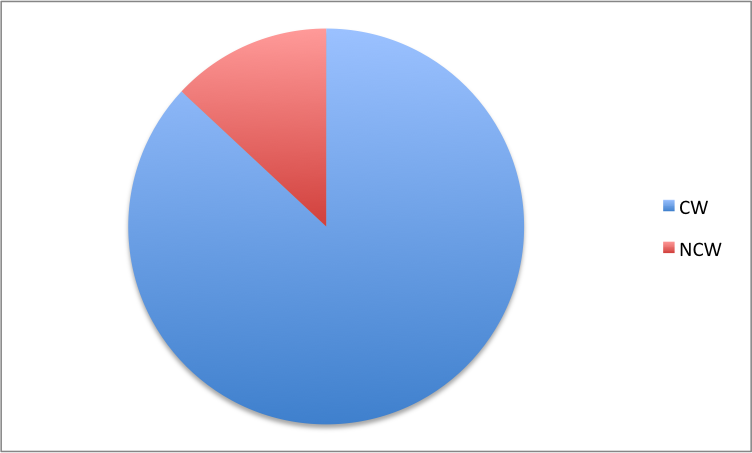
\includegraphics[height=2in]{figures/predictionAccuracy.png}
	\caption{Prediction accuracy in terms of which variant provided more appropriate clothes.}
	\label{fig:predictionAccuracy}
\end{figure}

\subsection{Decision Efficiency} \label{sec:results_de}

The quantitative measurements for decision effort were broken down into the number of critiquing cycles and the time it took to complete a recommendation session.

\subsubsection{Critiquing Cycles} \label{sec:results_de_cc}

Figure \ref{fig:critiquingCycles} shows the box plot of critiquing cycles for CW and NCW. It can be observed that the box of CW is obviously lower than the box of NCW, which suggests a difference between CW and NCW in critiquing cycles with cycles of CW being generally smaller than the ones of NCW. The mean of critiquing cycles for CW (2.83 cycles) is also smaller than the one for NCW (3.43 cycles) in Table \ref{tab:overview} but the difference is not significant (p=0.171). It can also be found that the box of NCW is comparatively shorter than the box of CW which suggests that some of the critiquing cycles of CW varies more than the ones of NCW. This can also be reflected from the standard deviations of critiquing cycles of these two variants in Table \ref{tab:overview} (2.46 for CW compared to 2.35 for NCW).

\begin{figure}[H]
	\centering
	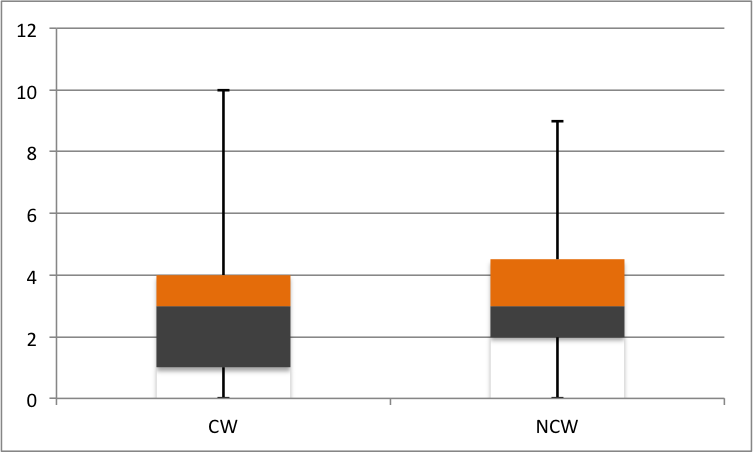
\includegraphics[height=2in]{figures/critiquingCycles.png}
	\caption{Decision efficiency in terms of critiquing cycles.}
	\label{fig:critiquingCycles}
\end{figure}

\subsubsection{Critiquing Time} \label{sec:results_de_ct}

Figure \ref{fig:critiquingTime} shows the box plot of critiquing time for CW and NCW. It can be observed that the medium of CW (109 seconds) is larger than the one of NCW (81 seconds), but the the box length of CW is comparatively shorter than the one of NCW, which suggests that the majority of the critiquing time of CW is more stable and is neither too long nor too short. For both two variants, the maximum (302 seconds for CW and 297 seconds for NCW) and minimum  (26 seconds for CW and 18 seconds for NCW) critiquing time are almost the same. 
From Table \ref{tab:overview}, it can be seen that from a general view, the critiquing time of CW varies more than that of NCW. NCW slightly beats CW in critiquing time when looking at the average time in Table \ref{tab:overview}, however, NCW is not significantly better.

\begin{figure}[H]
	\centering
	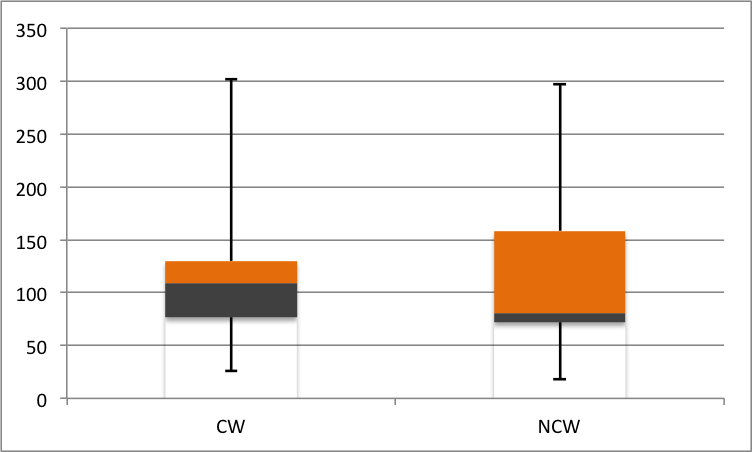
\includegraphics[height=2in]{figures/critiquingTime.png}
	\caption{Decision efficiency in terms of critiquing time.}
	\label{fig:critiquingTime}
\end{figure}

The qualitative measurements of decision efficiency were broken down into the rate for the ease of use of the system and the rate for the effectiveness of the system from the users.

\subsubsection{Ease of Use} \label{sec:results_de_eu}

To measure the ease of use of the system, the user was asked was it easy to find the information she/he needed (Q1). Whether or not useful information can be easily found depends on both the design of the recommendation approach and the design of the interface. When looking at the mean of the rate of this question in Table \ref{tab:overview}, CW slightly beats NCW (3.74 against 3.61). However the difference is not significant enough (p=0.3). The standard deviation of CW (0.92) is smaller than the one of NCW (1.16), which suggests that users have a higher level of agreement on the mean rate of CW.

When looking at Figure \ref{fig:easeOfUse}. It can be seen that more users gave score five for NCW than for CW (seven people for NCW and six people for CW). However, four people also gave negative rates for NCW (value 2), which did not appear to CW. Quite a number of people (9 people) hold a neutral view towards NCW compared to CW (6 people).

\begin{figure}[H]
	\centering
	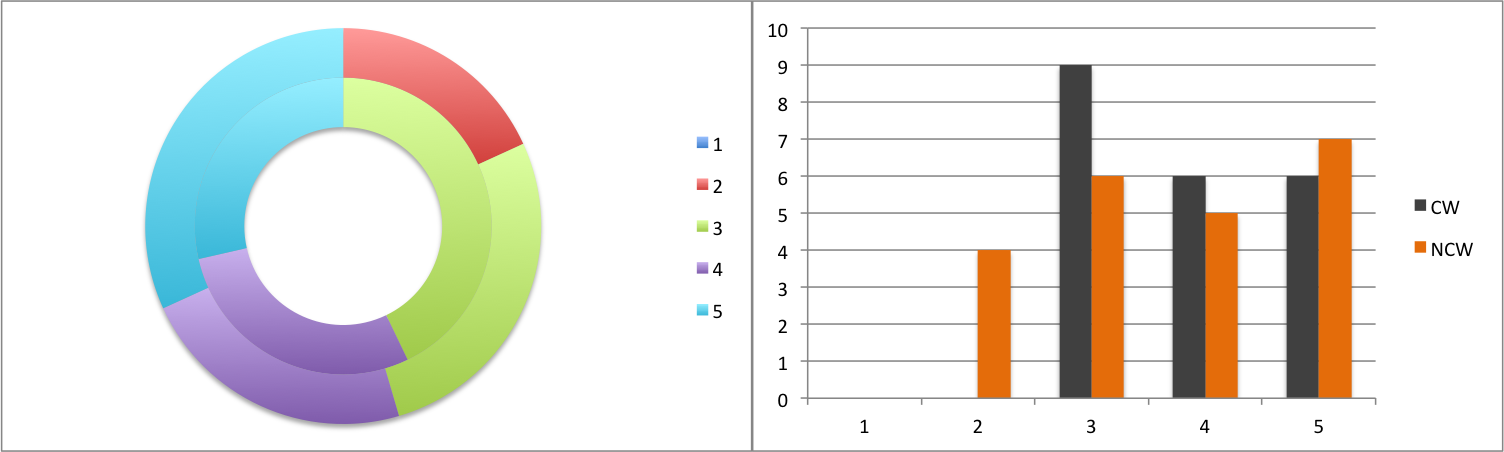
\includegraphics[height=1.7in]{figures/easeOfUse.png}
	\caption{Decision efficiency in terms of distribution of ratings for ease of use on a 5 point Likert scale (1, worst to 5, best). a) CW inner, NCW outer b) CW left, NCW right}
	\label{fig:easeOfUse}
\end{figure}

\subsubsection{Effectiveness} \label{sec:results_de_e}

To measure the effectiveness of the system, the user was asked the question was the system effective in helping her/him to complete the scenario (Q2). In the evaluation, the user was given a context scenario and was asked to imagine her/himself being in the context scenario while using the system. With this context-aware scenario, CW was rated significantly better than NCW (p=0.029 < 0.1). Some users mentioned that they found the context settings quite useful during the test. The average rate of CW (4.09) is also higher than that of NCW (3.74). On the other hand, the standard deviation of CW (0.79) is smaller than that of NCW which suggests that users had a higher degree of agreement towards the rating of CW than NCW.

If we look at Figure \ref{fig:effectiveness}, CW collected twice the number of positive (value 4 on the Likert scale) ratings and three quarters of the number of neutral ratings (value 3) compared to NCW. Also NCW received a negative ratings (value 2), while CW obtained a shared positive view.

\begin{figure}[H]
	\centering
	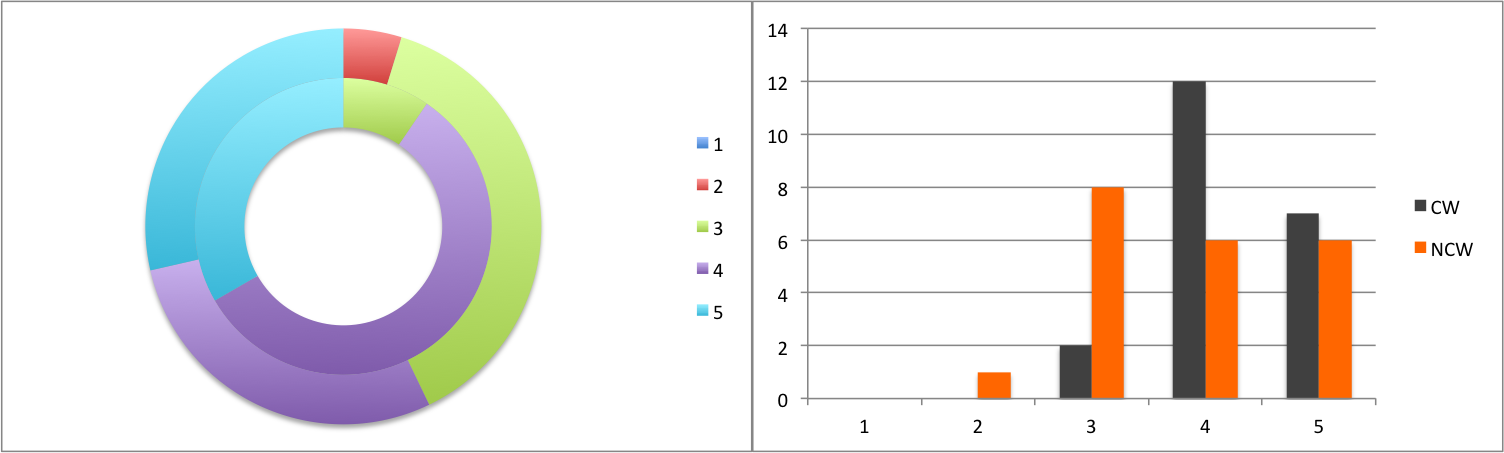
\includegraphics[height=1.7in]{figures/effectiveness.png}
	\caption{Decision efficiency in terms of distribution of ratings for effectiveness on a 5 point Likert scale (1, worst to 5, best). a) CW inner, NCW outer b) CW left, NCW right}
	\label{fig:effectiveness}
\end{figure}

\subsection{Context Benefits} \label{sec:results_cb}

To investigate whether users intuitively understood the benefits of using contextual information for recommendation but not seeing it as an obstruction, users were asked whether they understood the benefits of using the contextual conditions (Q4). In Figure \ref{fig:contextBenefits}, it can be seen that a majority of users (91\%, 21 people) gave positive ratings to this question and no negative ratings (value 1-2) were given.

\begin{figure}[H]
	\centering
	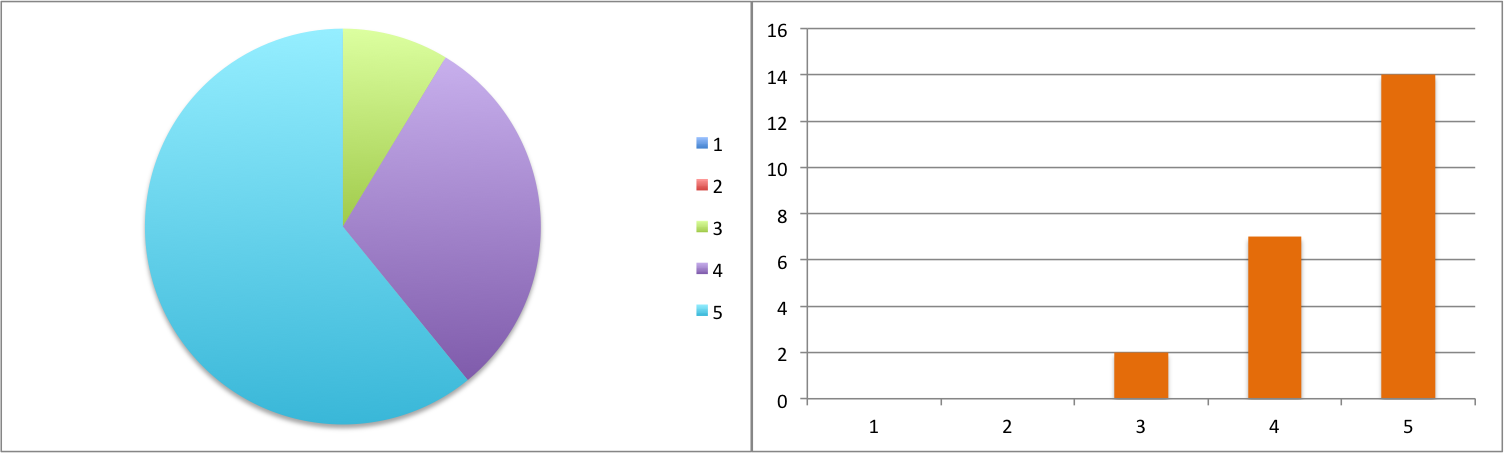
\includegraphics[height=1.7in]{figures/contextBenefits.png}
	\caption{Distribution of ratings for understanding of using contextual information on a 5 point Likert scale (1, worst to 5, best).}
	\label{fig:contextBenefits}
\end{figure}

\subsection{Explanation Benefits} \label{sec:results_eb}

Explanations for critiquing exist in both variants of the system. For the context-aware recommender system built in this thesis, another explanation was added in the detail page for each item to explain why an item was recommended using the contextual information. In this evaluation, it was investigated in particular the satisfaction, usefulness and clearness of this newly added explanation for the context-aware variant.

\subsubsection{Satisfaction} \label{sec:results_eb_s}

To test the general satisfaction of the contextual explanation, users were asked to rate how much were they satisfied with the provided contextual explanations (Q5). The average rating of satisfaction is 4.1. In Figure \ref{fig:satisfaction}, it can be seen that a majority of people (83\%, 19 people) gave positive ratings (value 4-5) and no negative ratings (value 1-2) were given. However, among the positive ratings, more users (13 people) gave a more conservative rating (value 4) rather than the most positive rating (value 5).

\begin{figure}[H]
	\centering
	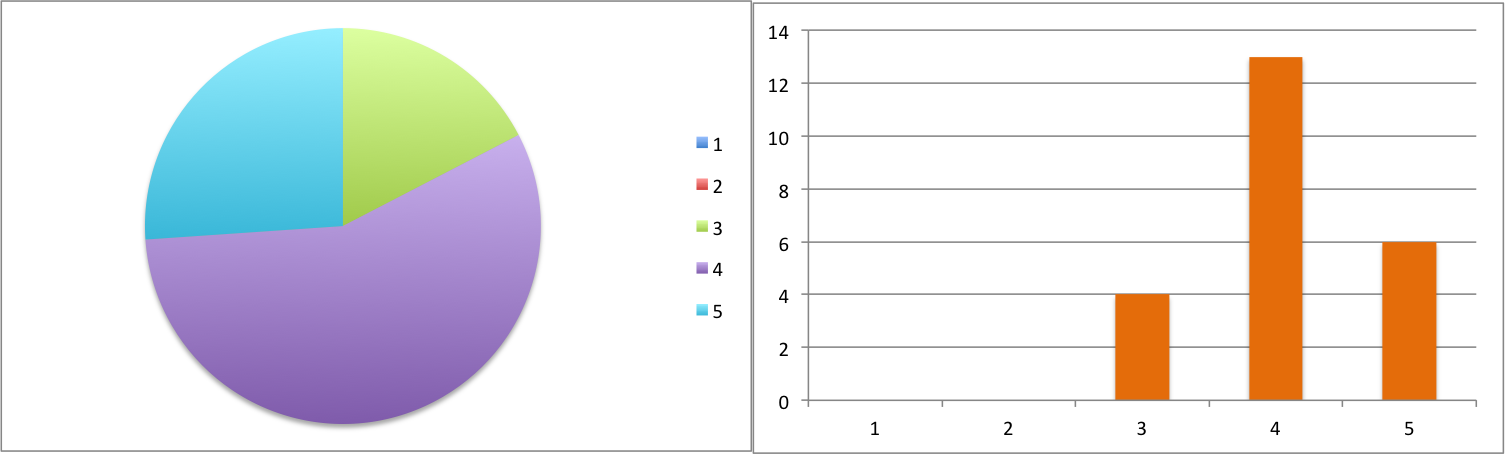
\includegraphics[height=1.7in]{figures/satisfaction.png}
	\caption{Explanation benefits in terms of distribution of ratings for satisfaction on a 5 point Likert scale (1, worst to 5, best).}
	\label{fig:satisfaction}
\end{figure}

\subsubsection{Usefulness} \label{sec:results_eb_u}

To test the usefulness of the provided contextual explanations, users were asked to rate how much did they believe that the contextual explanations were useful (Q6). The average rating of usefulness is 4.3, which is larger than the average rating of satisfaction. In Figure \ref{fig:usefulness}, it can be seen that a majority of people (83\%, 19 people) gave positive ratings (value 4-5) and no negative ratings (value 1-2) were given. Among the positive ratings, more people gave the most positive rating (value 5).

\begin{figure}[H]
	\centering
	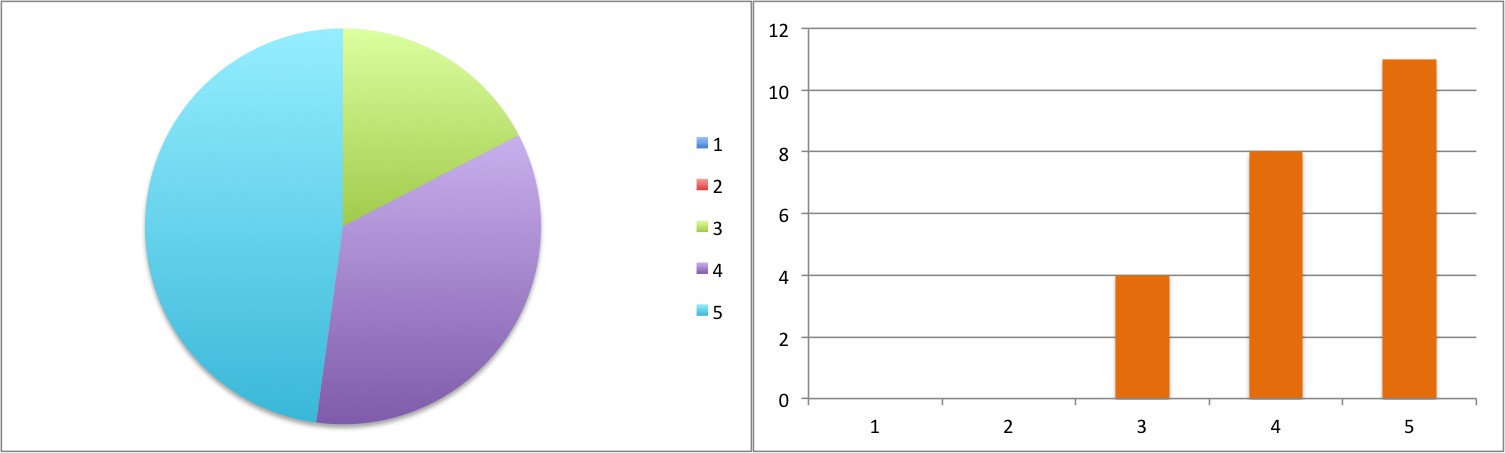
\includegraphics[height=1.7in]{figures/usefulness.png}
	\caption{Explanation benefits in terms of distribution of ratings for usefulness on a 5 point Likert scale (1, worst to 5, best).}
	\label{fig:usefulness}
\end{figure}

\subsubsection{Clearness} \label{sec:results_eb_c}

To measure the clearness of the contextual explanation, users were asked to rate how clear were the contextual explanations provided by the system (Q7). The average rating of the clearness is 4.4. In Figure \ref{fig:clearness}, it can be seen that a majority of people (78\%) gave positive ratings (value 5). Among the positive ratings, 77\% of the people gave the most positive ratings. Also no negative ratings (value 1-2) were given. 

\begin{figure}[H]
	\centering
	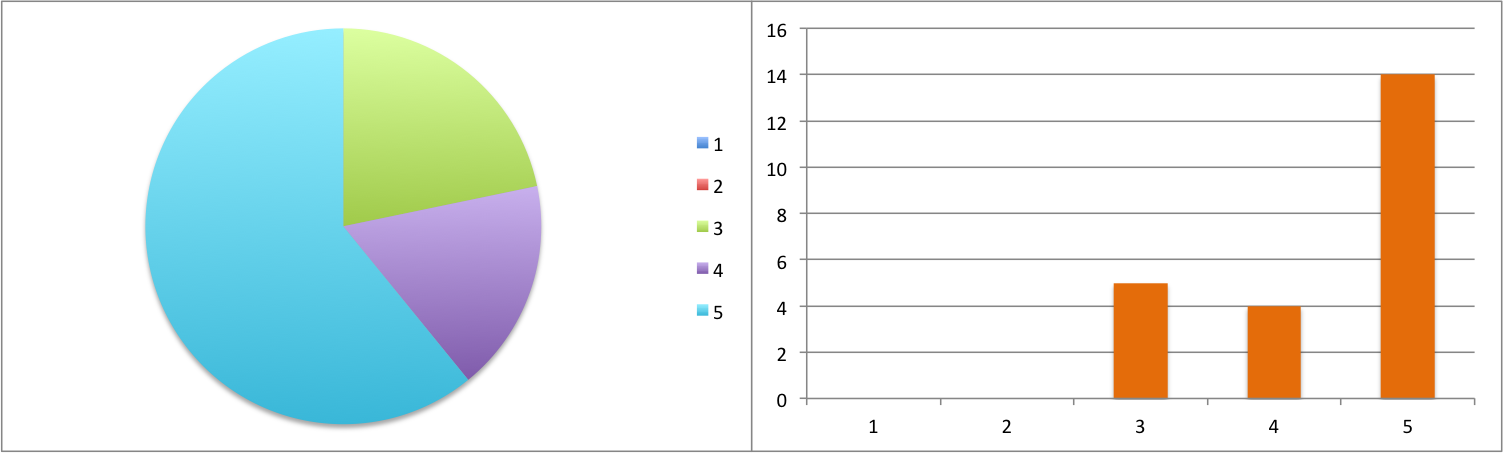
\includegraphics[height=1.7in]{figures/clearness.png}
	\caption{Explanation benefits in terms of distribution of ratings for clearness on a 5 point Likert scale (1, worst to 5, best).}
	\label{fig:clearness}
\end{figure}

\subsection{System Preference} \label{sec:results_sp}

\subsubsection{General Preference} \label{sec:results_sp_gp}

To investigate the system preferences, users were asked to choose which system they preferred more (Q8). In Figure \ref{fig:generalPreference}, it can be seen that 91\% people (21 people) preferred CW to NCW. Among the two people who selected NCW, one of them still preferred CW when they were asked to choose which system provided more appropriate clothes.

\begin{figure}[H]
	\centering
	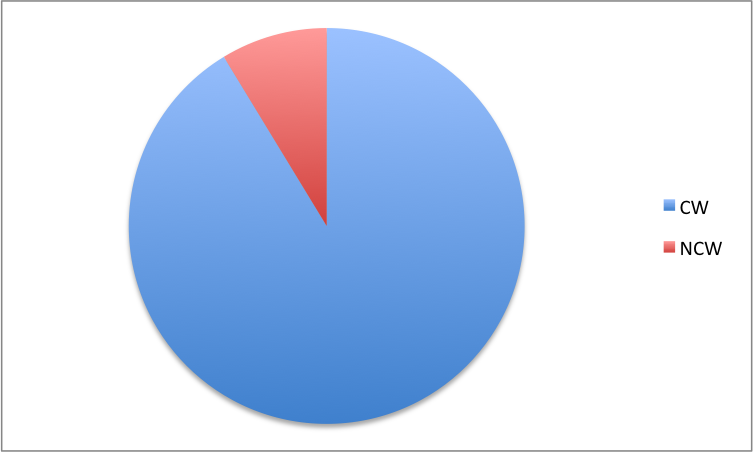
\includegraphics[height=2in]{figures/generalPreference.png}
	\caption{System preference in terms of distribution of general preference.}
	\label{fig:generalPreference}
\end{figure}


\subsubsection{Satisfaction} \label{sec:results_sp_s}

Users were also asked to give a specific rating of how much did they like using these two systems to provide a more detailed view (Q3). In Table \ref{tab:overview}, it can be seen that the mean rate of CW is higher than the one of NCW by about 0.65 and the difference is significant (with p = 0.004 < 0.1). Also the standard deviation of CW is smaller than NCW, which suggests that the users agreed more to the ratings of CW variant.

In Figure \ref{fig:systemSatisfaction}, it can be seen that users shared a positive view towards CW and no negative ratings were given to CW, while two negative ratings were given to NCW. When looking at the distribution of the positive ratings, CW collected twice the number of very positive ratings (value 5) and twice the number of positive ratings (value 4) compared to NCW variant. 

\begin{figure}[H]
	\centering
	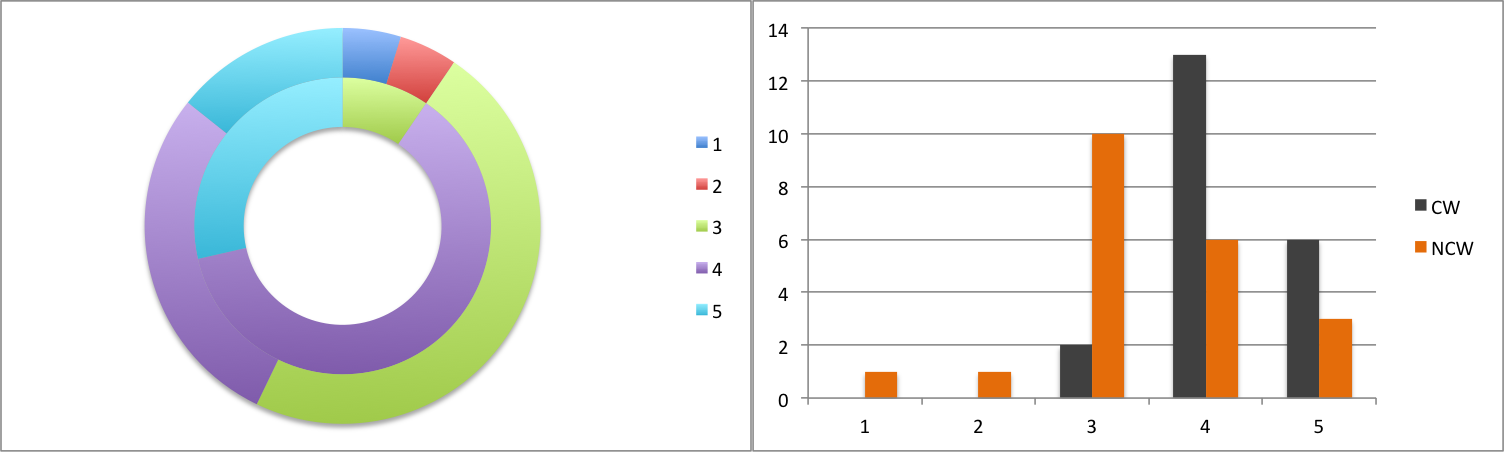
\includegraphics[height=1.7in]{figures/systemSatisfaction.png}
	\caption{System preference in terms of distribution of ratings for system satisfaction on a 5 point Likert scale (1, worst to 5, best). a) CW inner, NCW outer b) CW left, NCW right}
	\label{fig:systemSatisfaction}
\end{figure}

\subsection{Informal Feedback} \label{sec:results_if}

During the test, users were encourage to give informal feedback, because it is user's most direct feelings of the system and can be used as guidance for further improvements of the system. Here summarizes the most relevant and most interest views here.

\textbf{Allow manual input of the values for all available context factors.} Two participants mentioned that they might not always want to buy clothes under the current context. It was also possible that they wanted to buy for future context. Thus the system should not automatically retrieve values for context factors such as weather, temperature, but let the user enter the value by her/himself. The system can also be designed to allow the user to choose whether to let the system automatically detect the context value or let the user enter the value by her/himself.

\textbf{Improve the explanation through using icons and color.} From previous analysis, it can be seen that users value the usefulness of contextual explanations. There was a user who mentioned that instead of using only text, icons and different colors could also be used for displaying explanations because mages and colors were quicker than words and they could especially help to improve the user experience in mobile scenario.
 
\textbf{Put location information in more conspicuous place.} One user suggested that location, as a special context information, should be placed at a more conspicuous place (e.g., in the grid view where the user sees the list of all recommendations), because he thought that users were usually sensitive to location information.  

\textbf{Add a refresh button.} The system was built to display nice items for each cycle of recommendation. A few participants pointed out that a fresh button could be added. Instead of critiquing, they might want the system to show more items recommended based on the contextual information. It can be seen from here that the users valued the benefits of context and would like to rely more on it for recommendations.

\subsection{Correlation Analysis} \label{sec:results_ca}

To understand the relationship between different measurements instead of only interpreting single ones, a correlation analysis was performed on the measured data using the Pearson correlation coefficient. The correlation coefficient, denoted as r, measures the linear relationship between two variables and varies numerically between -1.00 and 1.00. The closer the value of r to 0, the weaker the relationship between the two variables is, with value 0 indicating an absence of relationship. The closer the value of r to 1 or -1, the stronger the relationship between the two variables is, with 1 indicating a perfect positive linear relationship and -1 indicating a perfect negative linear relationship. The values for all calculated r can be seen in Table \ref{tab:correlation}.

It can be seen that larger critiquing cycles is correlated with longer completion time (r=0.78). However, critiquing cycles and completion time are not correlated with the ease of use (r=0.04 for critiquing cycle, r=-0.11 for critiquing time), effectiveness (r=-0.08 for critiquing cycle, r=0.02 for critiquing time) and system satisfaction (r=-0.08 for critiquing cycle, r=-0.06 for critiquing time). Higher rating for system effectiveness is correlated with higher satisfaction of the system (r=0.5). 

When looking at the context benefits, it can be seen that the perceived benefits of using contextual conditions is not related to the general satisfaction of the current system (r=0.04). It is also not related to the clearness and the general satisfaction of the current system's explanation (r=0.08 for explanation satisfaction, r=0.18 for explanation clearness). So it can be suggested that user's preference of using contextual conditions is stable.

\begin{table}[H]
	\centering
	\caption{The correlation analysis.}
	\label{tab:correlation}
	\small
	\begin{tabular}{p{1.2in}p{0.3in}p{0.3in}p{0.3in}p{0.3in}p{0.3in}p{0.3in}p{0.3in}p{0.3in}p{0.3in}}
	          \hline
		 & EoU & E & SS & CB & ES & EU & EQ & CC & CT \\ \hline
		Ease of Use & 1 & 0.56 & 0.25 & 0.08 & 0.11 & 0.05 & 0.08 & 0.04 & -0.11 \\
		Effectiveness &  & 1 & 0.5 & 0.08 & -0.1 & 0.03 & 0.36 & -0.08 & 0.02 \\
		System Satisfaction &  &  & 1 & 0.04 & 0.08 & 0.05 & 0.18 & -0.08 & -0.06 \\
		Context Benefits &  &  &  & 1 & 0.3 & 0.48 & 0.27 & -0.08 & -0.27 \\
		Explanation Satisfaction &  &  &  &  & 1 & 0.48 & 0.42 & 0.01 & -0.03 \\
		Explanation Usefulness &  &  &  &  &  & 1 & 0.59 & 0.1 & 0 \\
		Explanation Clearness &  &  &  &  &  &  & 1 & 0.06 & 0.19 \\
		Critiquing Cycle &  &  &  &  &  &  &  & 1 & 0.78 \\
		Completion Time &  &  &  &  &  &  &  &  & 1 \\ \hline
	\end{tabular}
\end{table}

\section{Discussion} \label{sec:discussion}

Regarding prediction accuracy, the majority of people thought that context-aware variant CW showed more appropriate clothes than non context-aware variant. According to some informal feedbacks, clothes presented in CW looked better than those presented in NCW for the users. It might be because CW was recommending based on user's contextual information as initial preferences and could filter out clothes that were not satisfying. Also the clothes in the case base of CW were carefully selected manually according to expert knowledge, clothes with good design and cheaper cost could be discovered using collaborative effort which helped with raising the recommendation accuracy.

Regarding ease of use, CW slightly beats NCW by 0.13, but the difference is not significant (p=0.3). However, users shared a positive view towards CW but gave 4 negative ratings (value 2) to NCW. It might be because users were give a way to express their contextual requirements and thus found the CW variant be more multifunctional and powerful. But it should also be noted that a too complicated user interface or unclear recommendation logic will also make the users be confused and rate the system low.

Regarding system effectiveness, CW significantly beats NCW by 0.35 (p=0.029). Since the users were asked to imagine a contextual scenario, users were more aware of the contextual requirement and thus valued the context-aware recommendation more. There was one time, when the user was shown the context setting interface, the user commented that it was the exact thing he was looking for. On the other hand, more users gave positive ratings (value 4) than most positive ratings (value 5). It might be caused by their dissatisfaction of the missing of some other recommendation approaches that can always be seen in the online recommendation systems like Amazon. Some users commented that the system should allow the user to select the clothes category and gender first. Some other users would like to have a refresh button so that they can update the recommendations using the current context settings without critiquing.

Regarding context benefits, it is interesting to notice that the users all shared a positive view towards using context for recommendation and users gave twice the number of most positive ratings (value 5) compared to positive ratings (value 4). Thus it can be suggested that users are not against to using contextual information. In the correlation analysis, it is shown that user's preference of using contextual information was not related to the clearness and satisfaction of the current system's explanation. Thus it was not the special design of the system that highlighted the importance of context and it can be suggested that users are expecting recommender systems that can recommend based on their current context. 

Regarding the contextual explanations, it is shown that users shared a positive view towards the provided contextual explanations. The usefulness of the contextual explanation was scored high (average = 4.30), but the satisfaction of the explanation was scored a little bit lower (average = 4.09). It can be suggested that the importance of contextual explanations is valued high and users are quite sensitive to the quality of the explanations. The quality of the explanation can not be measured only by clearness, which can be indicated from the high score obtained by clearness (average = 4.39). 

Finally, regarding system preference, more participants preferred using CW over NCW and significantly more participants were generally more satisfied with CW than NCW. Also a close relation was detected between system satisfaction and system effectiveness. It might be because for mobile application, users are more sensitive to the effectiveness of the system and the system effectiveness thus influences the general satisfaction of the system more than usual. Overall, the developed context-aware recommender system was proved to have successfully integrated contextual information into the conversation-based Active Learning system using case-based recommendation approach. 

















































